\documentclass[a4paper,12pt]{article}

\usepackage[utf8]{inputenc} 
\usepackage{amsmath}
\usepackage[a4paper, margin=0.9in]{geometry} % Adjust the margin here
\usepackage{multirow}
\usepackage{graphicx}
\usepackage{tikz}
\usepackage{wrapfig}

\begin{document}


\section*{Question 1}

\begin{wrapfigure}{r}{0.35\textwidth}
    \centering
    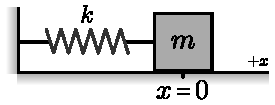
\includegraphics[scale=1]{figures/ho.pdf}
\end{wrapfigure}

A block is attached to the wall with a spring as it is shown in the figure. $k$ is the spring constant, $m$ is the mass of the body and $x=0$ is the equilibrium point of the system. It is given that the spring and all connection equipment are massless and the system is completely frictionless. We will only consider very small oscillations so that $x\ll 1$.
\begin{itemize}
    \item [\textbf{(a)}] Sketch the free-body diagrams of the block for $x>0$, $x=0$ and $x<0$. --- \textit{0.2 points}
    \item[\textbf{(b)}] Write down the equation of the motion (Newton's 2nd Law) of the block in differential equation form but do not solve it. Write the oscillation frequency $\omega_0$ in terms of $k$ and $m$. --- \textit{0.2 points}
    \item[\textbf{(c)}] By using the solution assumption $x(t)=e^{\lambda t}$ solve the equation of motion in \textbf{(b)} and write down the solution in $x(t)=Ae^{-i\omega_0 t}+Be^{i\omega_0 t}$ form, where $A$ and $B$ are some arbitrary constants. --- \textit{0.6 points}
\end{itemize}
\section*{Question 2}
A particle of mass $m$ moves under the influence of a central force $\vec{F}(r)=-\frac{k}{r^3}\hat{r}$, where $k$ is and arbitrary constant and $r$ is the radial distance from the origin.

\begin{itemize}
    \item[\textbf{(a)}] Explain in very simple terms why the angular momentum of the particle is conserved. --- \textit{0.4 points}
    \item[\textbf{(b)}] The effective potential of the particle is given as $V(r)=U(r)+\frac{l^2}{2mr^2}$, where $U(r)$ is the potential of the particle and $l=mr^2\dot{\theta}$ is the angular momentum. Express $V(r)$ in terms of $k$, $l$, $m$ and $r$. --- \textit{0.6 points}
\end{itemize}

\section*{Question 3}
A pendulum is suspended inside an uniformly accelerating train with $a_0$ moving along a straight horizontal track. Express the angle $\theta$  that the pendulum makes with the vertical in the accelerating frame (in the train) in terms of $a_0$ and $g$, where $g$ is the gravitational acceleration. --- \textit{1 point}

\section*{Question 4}
Consider a system of three point particles, each having an identical mass $m$, with their positions defined by time-dependent vectors,
\begin{equation*}
    \vec r_{1}~=~(at^2,~vt,~0),~\vec r_{2}~=~(vt,~at^2,~b),~\vec r_{3}~=~(0,~b,~at^2), 
\end{equation*}
where $a$, $b$, and $v$ are positive constants. Determine the total external force and the total torque exerted on this system concerning the origin of coordinates. Additionally, based on these findings, analyze whether the system conserves linear and angular momentum.

\end{document}
